\documentclass[12pt,a4paper]{article}

\usepackage[cm]{fullpage}
\usepackage{amsthm}
\usepackage{amsmath}
\usepackage{amsfonts}
\usepackage{amssymb}
\usepackage{xspace}
\usepackage[english]{babel} % Used for date formatting
\usepackage{fancyhdr}
\usepackage{titling}
\usepackage{url}
\usepackage{csquotes}
\usepackage[
    style=numeric,
    bibstyle = numeric,
    citestyle = numeric,
    sorting = none,
    backend=biber
]{biblatex}
\usepackage{parskip}
\usepackage{graphicx}
\usepackage{subcaption}
\usepackage{hyperref}
\usepackage{listings}
\usepackage[table,xcdraw]{xcolor}
\usepackage{nameref}
\graphicspath{ {./img/} }
\addbibresource{summary.bib}

\usepackage{multirow}
\usepackage{listings}

\usepackage{mdframed}
\usepackage{lipsum}

\newmdtheoremenv{theo}{Theorem}

%%%%%%%%%%%%%%%%%%%%%%%%%%%%%%%%%%%%%%%%%
% - Declare some maths operators
%%%%%%%%%%%%%%%%%%%%%%%%%%%%%%%%%%%%%%%%%
\DeclareMathOperator*{\argmax}{argmax}

%%%%%%%%%%%%%%%%%%%%%%%%%%%%%%%%%%%%%%%%%
% - Format date to ''dd.mm.YYYY''
%%%%%%%%%%%%%%%%%%%%%%%%%%%%%%%%%%%%%%%%%
\DefineBibliographyExtras{english}{%
  \protected\def\mkbibdateshort#1#2#3{%
    \iffieldundef{#3}
      {}
      {\mkdayzeros{\thefield{#3}}%
       \iffieldundef{#2}{}{.}}%
    \iffieldundef{#2}
      {}
      {\mkmonthzeros{\thefield{#2}}%
       \iffieldundef{#1}{}{.}}%
    \iffieldbibstring{#1}
      {\bibstring{\thefield{#1}}}
      {\dateeraprintpre{#1}\mkyearzeros{\thefield{#1}}}}%
  \protected\def\mkbibdatelong#1#2#3{%
    \iffieldundef{#3}
      {}
      {\stripzeros{\thefield{#3}}%
       \iffieldundef{#2}{}{\nobreakspace}}%
    \iffieldundef{#2}
      {}
      {\mkbibmonth{\thefield{#2}}%
       \iffieldundef{#1}{}{\space}}%
    \iffieldbibstring{#1}{\bibstring{\thefield{#1}}}{\stripzeros{\thefield{#1}}}}%
}


%%%%%%%%%%%%%%%%%%%%%%%%%%%%%%%%%%%%%%%%%
% - Define LST-LISTINGS
%%%%%%%%%%%%%%%%%%%%%%%%%%%%%%%%%%%%%%%%%
\definecolor{backcolor}{rgb}{0.95,0.95,0.92}

\lstdefinestyle{mystyle}{
    backgroundcolor=\color{backcolor},
    breaklines=true,
    numbers=left,
    numbersep=5pt,
    basicstyle=\ttfamily\footnotesize,
    captionpos=b
}

\lstset{style=mystyle}

%%%%%%%%%%%%%%%%%%%%%%%%%%%%%%%%%%%%%%%%%%
% This part needs customization from you %
%%%%%%%%%%%%%%%%%%%%%%%%%%%%%%%%%%%%%%%%%%

% your group number your names and matriculation numbers here
\newcommand{\groupnumber}{1}
\newcommand{\name}{From: Thinklex}
\newcommand{\matriculation}{To: The masses}
\newcommand{\gt}{\ensuremath >} 

%%%%%%%%%%%%%%%%%%%%%%%%%%%%%%%%%%%%%%%%%%
%           End of customization         %
%%%%%%%%%%%%%%%%%%%%%%%%%%%%%%%%%%%%%%%%%%

\newcommand{\projnumber}{1}
\newcommand{\Title}{Summary}
\setlength{\headheight}{15.2pt}
\setlength{\headsep}{20pt}
\setlength{\textheight}{680pt}
\pagestyle{fancy}
\fancyhf{} 
\fancyhead[L]{Machine Learning - Summary}
\fancyhead[C]{}
\fancyhead[R]{\name}
\renewcommand{\headrulewidth}{0.4pt}
\fancyfoot[C]{\thepage}


\begin{document}
\thispagestyle{empty}
\noindent\framebox[\linewidth]{%
 \begin{minipage}{\linewidth}%
 \hspace*{5pt} \textbf{Machine Learning (SS2022)} \hfill TU Wien
 \hspace*{5pt}\\

 \begin{center}
  {\bf\Large Summary}
 \end{center}

 \vspace*{5pt}\hspace*{5pt} 29.06.2022\hfill Summary ML\hspace*{5pt}
\end{minipage}%
}
\vspace{0.5cm}
%%%%%%%%%%%%%%%%%%%%%%%%%%%%%%%%%%%%%%%%%%%%%%%


\begin{center}
\textbf{\name} %please fill the information above

\matriculation %please fill the information above
\end{center}
%%%%%%%%%%%%%%%%%%%%%%%%%%%%%%%%%%%%%%%%%%%%%%%

\section{Preliminaries}

\noindent This summary is for the Machine Learning course of the Vienna University of Technology and was initially created for the Summer Term 2022 in a process of studying for the exam. Most of the basic subjects are covered in depth in this summary, but some of the more advanced topics (like SVM or Reinforcement Learning) are not covered in depth.\\
This summary is available on GitHub, if you find typos, errors, want to add something (content, links, figures, ...) or just want to contribute you can do this here: \url{https://github.com/alexl4123/ml-summary}.\\
If the URL doesn't work, you can find it in GitHub if you search for:
\begin{itemize}
    \item User: alexl4123
    \item Repo-Name: ml-summary
\end{itemize}

\newpage
\section{Introduction, Data stuff and Experiments}

\noindent Machine Learning (ML) is a subfield of a field which is generally known as ''Artificial Intelligence'', whereas Machine Learning is the subdiscipline which \textit{studies algorithms that can learn from data and make predictions on data}. Machine Learning can further be subdivided into three fields:
\begin{itemize}
    \item \textit{Unsupervised-ML}: Generally wants to find structure in unlabeled data, has many words which are sometimes used as synonyms, like \textit{Data Mining}. Also Multivariate-Statistics has a many unsupervised techniques, like Principal-Component-Analysis (PCA), which can be used for dimensionality reduction.
    \item \textit{Supervised-ML}: \textbf{Is the main topic of this class}, although some other methods of ML are also taught. This subdiscipline tries to predict \textit{unknown data}, by observing \textit{known} data. Sometimes \textit{offline-learning} is used as a synonym for supervised learning, which underscores the fact, that for a supervised method the data must be known in advance to learn from it. Supervised methods are generally subdivided into \textit{classification}, which tries to predict classes, and \textit{regression}, which tries to predict numeric values.
    \item \textit{Reinforcement-Learning (RL)}: This process of learning is inspired by nature, i.e. how most animals learn, e.g. one does not touch a hot plate twice (except one is a scientist...). Other names for RL are \textit{online-learning}, which highlights the point, that learning is done repeatedly, and one more name is \textit{trial-and-error-learning}, which tries to point out, that one needs to try out certain actions, which may fail, to learn something. The \textit{exploitation-exploration} dilema is the most present one in this are of learning.
\end{itemize}

\noindent As some names are sometimes used in multiple occasions, the following list provides some terminology which is required for the lecture:

\begin{itemize}
    \item \textit{Feature}: A column of the dataset table.
    \item \textit{Observation}: A row of the dataset table.
    \item \textit{Model}: The model is the algorithm, which is used for the machine-learning process.
    \item \textit{Model-Fitting}: A model is fitted (aka. trained) with some data, to make sense of the data.
    \item \textit{Prediction}: Given a fitted model, one can use unlabeled data to predict the labels.
    \item \textit{Hyper-Parameters}: Hyper-Parameters are the parameters which are used by the model. E.g. for a Neural-Network this is the amount of layers and neurons per layer.
    \item \textit{Performance of Model}: Can either be the \textit{effectiveness}, i.e. the value of the performance measure, or the \textit{efficiency}, i.e. the computational cost. In the lecture and in this summary performance is mostly used as a synonym for effectiveness.
\end{itemize}

\noindent The general process for analyzing data and making sense of it can be viewed in the \textit{Data Science Process}, which basically has five steps:

\begin{enumerate}
    \item \textbf{Ask} a question: \textit{What is the scientific goal?}, \textit{What do you want to predict or estimate?},...
    \item \textbf{Get} the data: \textit{How were the data sampled?}, \textit{Which data are relevant?},...
    \item \textbf{Explore} the data: \textit{Plot the data}, \textit{Are there anomalies?},...
    \item \textbf{Model} the data: \textit{Build the model}, \textit{fit the model}, \textit{evaluate the model},...
    \item \textit{Communicate and visualize the results}.

\end{enumerate}

\subsection{Data}

\noindent This lecture considers four types of data:

\begin{itemize}
    \item \textit{Nominal}: Values are distinct symbols, like ''green'', ''blue'', etc. Is regarded as a \textit{qualitative} data. Relation or arithmetic operations do not make sense on this data type.
    \item \textit{Ordinal}: Values have a rank among them, like ''large'' \(>\) ''medium'' \(>\) ''tiny''. Therefore order computations make sense, but distance measure or most of the other arithmetic operators do not. Is regarded as a \textit{qualitative} data type.
    \item \textit{Interval}: Are ordered and measured in fixed and equal units, therefore distance measurement makes sense, but most arithmetic operations do not (like multiplication, etc.). Is regarded as a \textit{quantitative} data type. An example is for instance temperature measured in degree celcius (e.g. 20 degrees are not twice as warm as 10 degrees).
    \item \textit{Ratio}: Are ordered, distance measurements make sense and most arithmetic operations make sense. An example is e.g. temperature measured in kelvin, because e.g. 273.15 kelvin are twice as ''warm'' as 136.575 kelvin. Is regarded as a \textit{quantitative} data type.
\end{itemize}

\subsubsection{Scaling/Normalization/Standardisation}

\noindent If multiple quantitative features are present in a dataset, then they may exhibit vastly different value ranges. This might be a problem, if a model is based on the difference between values of different features. Therefore in these problems, one must scale the features, which can be done in various different ways. Some methods which can be used include:
\begin{itemize}
    \item Log-Transforming each feature, i.e.: \(z_i = log(x_i)\)
    \item Min-Max-Scaling: \(z_i = \frac{x_i - min(x)}{max(x) - min(x)}\). Transforms value range to \([0,1]\).
    \item Z-score standardisation: \(z_i = \frac{x_i - \overline{x}}{s}\), where \(\overline{x}\) denotes the empirical expected value and \(s\) denotes the empirical standard deviation (square root of empirical variance). Transforms value range to \((-\infty, +\infty)\) with mean \(0\).
\end{itemize}

\subsubsection{Qualitative Data encondings}

\noindent If one has qualitative data, like the nominal feature eye-color, with values ''black'', ''pink'' and ''white'', then one has several options to proceed:

\begin{itemize}
    \item \textit{One-hot-encoding} (1-to-N Coding): For this the original feature vector ''eye-color'' is removed from the dataset and in our case three new vectors are introduced: ''black'', ''pink'' and ''white''. Each new vector is now a boolean vector, which denotes that a certain observation has or does not have the specific feature.
    \item \textit{Label-encoding}: Another possibility is to stick with the current feature ''eye-color'', but change the content to a numeric representation, e.g. associate ''black'' with \(0\), ''pink'' with \(1\) and ''white'' with \(2\), then change the nominal representation to the numeric one.
\end{itemize}

\subsubsection{Missing Values}

\noindent For some datasets not all values are known, e.g. a certain observation only has 9 of the 10 features. Standard procedures exists for this:

\begin{itemize}
    \item Deletion of feature (column), seems mostly to be a bad practice, as the feature might contain very important information for other observations (especially costly, if there are not many features).
    \item Deletion of observation (row), seems a better option than deleting the feature entirely, although sometimes also costly (if there are not many datapoints).
    \item Data imputation, seems to be a good idea, but value then only holds true to a certain extend. Popular measures for imputation are \textit{mean/median} value, \textit{random selection}, \textit{regression}, \textit{clustering} or \textit{nearest-neighbor} (so actually some super-/unsupervised methods).
\end{itemize}

\subsection{Experiments}

\noindent Generally from the experiment one should get a good estimation how well the model works. Therefore the main task of the experiment is to evaluate the model performance in terms of the performance measure, for which several different possibilities exist (see Classification and Regression).\\
The general structure of the experiment phase mostly consists of a \textit{training} and a \textit{test} phase. This is e.g. achieved by splitting the original dataset into two datasets, one for training and one for testing. This is done to get a good estimate how well the model works in real conditions with unseen data.\\
One method which tries to even get better estimates on the true model performance is \textit{Cross-Validation (CV)}. For this one repeatedly performs train-tests-splits of the data and averages the results. E.g. for a five-fold-CV one splits the data into five equal parts (each representing \(20\%\) of the data) and then performs five experiments. The first one uses the first four parts as the training data and the fifth part for testing. The second one uses the first three parts and the fifth part for training and the fourth for testing... this continues as long as a part has not been used for testing (i.e. 5 times). Then one averages the results to get the CV-score.\\[1em]
Another CV approach is \textit{leave-p-out CV}, which uses \(p\) observations in the test set. This method is mostly computational infeasable.

\subsubsection{Data Leakage}

\noindent In the experiment design it is important to mitigate the threat of data-leakage, which leaks information from the training set into the test set. This is bad, as so one cannot get a true estimate how well the model performs, therefore this has to be avoided.\\
Important is here, to perform methods like scaling not on the whole dataset, but on the test/train set individually.

\subsubsection{Experiment design for Hyper-Parameter-Tuning}

\noindent For this one should perform another split, e.g. \(60\%\) training set for HPP, \(20\%\) test set for HPP, \(20\%\) test set for sanity check.\\
So the HPP-tuning should be done on the first \(60/20\) split, after they HPPs have been selected then another check on the other \(20\%\) is performed.

\subsubsection{Stratification}

\noindent In the normal case, the train/test-split is performed completely random, which can lead to a situation where one class is not present in the train- or test-set. To mitigate this one can also use stratification. This method assures, that the classes are approximately equally represented in the test and in the train set.\\
The problem with this method is, that this might not reflect a real world scenario.

\subsubsection{Bootstrapping}
\label{subsubsec:bootstrapping}

\noindent A bootstrap is a random sample of a dataset, which was drawn by sampling with replacement, i.e. an observation might occur multiple times (or not at all) in a bootstrap-sample.

\subsection{Overfitting/Underfitting}

\noindent The overfitting/underfitting problem is a general supervised-ML problem. Overfitting means, that the model is trained so well on the training set, that it cannot generalize to unseen data. Underfitting in contrast means, that the algorithm didn't really learned anything at all and therefore needs to consider more datapoints.\\
If one has a good performance for the training set, but a bad performance for the test set, this accounts to overfitting. In contrast to that, underfitting usually shows bad performance in the training set as well as in the test set.\\[1em]
For this context also the \textit{bias} and \textit{variance} problemi/tradeoff arises. High \textit{bias} can be seen as something similar to underfitting, whereas high \textit{variance} is similar to overfitting. This is as, bias is an error fundamental to the assumptions of the data, whereas high variance is caused by small fluctuations in the data, which leads to big differences in the output.\\
The important thing here is, that bias and variance can simultaneously be high and minimizing both of them simultaneously is hard.

\newpage
\section{Classification}

\noindent A classification problem arises, when one wants to classify unseen data, e.g. the classification of a car maker according to visual features of the car.\\

\subsection{Performance Measures}

\noindent For classification problems, there are multiple performance measures. For a binary classification task one may choose between \textit{Accuracy}, \textit{Precision} and \textit{Recall}.

% Please add the following required packages to your document preamble:
% \usepackage{multirow}
% \usepackage[table,xcdraw]{xcolor}
% If you use beamer only pass "xcolor=table" option, i.e. \documentclass[xcolor=table]{beamer}
\begin{table}[h]
\begin{tabular}{ll|ll|l}
\cline{3-4}
                                                                                                                                       &       & \multicolumn{2}{l|}{\textbf{Actual value (groundtruth)}}                                                                                                                                                      &                                                                                                               \\ \cline{3-4}
                                                                                                                                       &       & \multicolumn{1}{l|}{true}                                                                                                 & false                                                                                               &                                                                                                               \\ \hline
\multicolumn{1}{|l|}{}                                                                                                                 & true  & \multicolumn{1}{l|}{\cellcolor[HTML]{95C884}\begin{tabular}[c]{@{}l@{}}True Positive \\ (TP)\end{tabular}}                & \cellcolor[HTML]{E49696}\begin{tabular}[c]{@{}l@{}}False Positive\\ (FP, Type I Error)\end{tabular} & \multicolumn{1}{l|}{Precision \(\frac{TP}{TP + FP}\)}                                                         \\ \cline{2-5} 
    \multicolumn{1}{|l|}{\multirow{-2}{*}{\begin{tabular}[c]{@{}l@{}}\textbf{Prediction /}\\ \textbf{Test outcome}\end{tabular}}} & false & \multicolumn{1}{l|}{\cellcolor[HTML]{E49696}\begin{tabular}[c]{@{}l@{}}False Negative\\ (FN, Type II Error)\end{tabular}} & \cellcolor[HTML]{95C884}\begin{tabular}[c]{@{}l@{}}True Negative\\ (TN)\end{tabular}                & \multicolumn{1}{l|}{}                                                                                         \\ \hline
                                                                                                                                       &       & \multicolumn{1}{l|}{\begin{tabular}[c]{@{}l@{}}Recall/Sensitivity\\ \(\frac{TP}{TP + FN}\)\end{tabular}}                  & \begin{tabular}[c]{@{}l@{}}Specificity\\ (True negative rate)\end{tabular}                          & \multicolumn{1}{l|}{\begin{tabular}[c]{@{}l@{}}Accuracy\\ \(\frac{TP + TN}{TP + TN + FP + FN}\)\end{tabular}} \\ \cline{3-5} 
\end{tabular}
\end{table}

\noindent Additionally the \textit{F1-Score} exists (seems not to be used in the lecture), which can be computed as:

\[F1 = 2 \cdot \frac{Precision \cdot Recall}{Precision + Recall}\]

\noindent There are also various other performance measures, which one can look up in the internet.

\subsubsection{Performance Measures for Multiclass Classification}

\noindent Again several options possible, the lecture presents \textit{micro-average}, \textit{macro-average} and \textit{costs of misclassification}. To understand those three performance measurements, have a look at the confusion table below (note that the ground truth is ''vertical'', which is consistent with the above notion, but in the lecture they switched it):

% Please add the following required packages to your document preamble:
% \usepackage{multirow}
% \usepackage[table,xcdraw]{xcolor}
% If you use beamer only pass "xcolor=table" option, i.e. \documentclass[xcolor=table]{beamer}
\begin{table}[h]
\begin{tabular}{cc|ccc|c}
\cline{3-5}
                                                    &                       & \multicolumn{3}{c|}{Groundtruth}                                                                                               &                          \\ \cline{3-6}
                                                    &                       & \multicolumn{1}{c|}{1}                          & \multicolumn{1}{c|}{2}                          & 3                          & \multicolumn{1}{c|}{Sum} \\ \hline
\multicolumn{1}{|c|}{}                              & 1                     & \multicolumn{1}{c|}{\cellcolor[HTML]{95C884}20} & \multicolumn{1}{c|}{\cellcolor[HTML]{E49696}10} & \cellcolor[HTML]{E49696}0  & \multicolumn{1}{c|}{30}  \\ \cline{2-6}
\multicolumn{1}{|c|}{}                              & 2                     & \multicolumn{1}{c|}{\cellcolor[HTML]{E49696}0}  & \multicolumn{1}{c|}{\cellcolor[HTML]{95C884}0}  & \cellcolor[HTML]{E49696}5  & \multicolumn{1}{c|}{5}   \\ \cline{2-6}
\multicolumn{1}{|c|}{\multirow{-3}{*}{Predictions}} & 3                     & \multicolumn{1}{c|}{\cellcolor[HTML]{E49696}5}  & \multicolumn{1}{c|}{\cellcolor[HTML]{E49696}10} & \cellcolor[HTML]{95C884}95 & \multicolumn{1}{c|}{110} \\ \hline
\multicolumn{1}{|c|}{Sum}                           &                       & \multicolumn{1}{c|}{25}                         & \multicolumn{1}{c|}{20}                         & 100                        & \multicolumn{1}{c|}{145}    \\ \hline
\multicolumn{1}{|l|}{Accuracy}                      & \multicolumn{1}{l|}{} & \multicolumn{1}{l|}{0.8}                         & \multicolumn{1}{l|}{0}                          & \multicolumn{1}{l|}{0.95}    & \multicolumn{1}{l|}{}    \\ \hline
\end{tabular}
\end{table}

\noindent \textbf{Micro-Average}: Can now be calculated, by summing up all true classifications of all cells and then divide by the total amount of observations. In the following the micro average for our example is calculated, where \(n\) resembles the amount of classes:

\[acc_{micro} = \frac{\sum_{i=1}^{n} TP_i}{\#samples} = \frac{20 + 0 + 95}{145} = 0.79\]

\noindent \textbf{Macro-Average}: Can be calculated, by averaging the accuracies of each individual class. Again the formula for our case is shown:

\[acc_{macro} = \frac{\sum_{i=1}^{n} acc_i}{n} = \frac{0.8 + 0 + 0.95}{3} = 0.58\]

\noindent \textbf{Costs of missclassification}: For this one must define another matrix, the \textit{cost matrix}, which defines how much a missclassification costs. In our case we assume different costs for different missclassifications:

% Please add the following required packages to your document preamble:
% \usepackage{multirow}
% \usepackage[table,xcdraw]{xcolor}
% If you use beamer only pass "xcolor=table" option, i.e. \documentclass[xcolor=table]{beamer}
\begin{table}[h]
\begin{tabular}{|cc|ccc|}
\hline
\multicolumn{2}{|c|}{}                                       & \multicolumn{3}{c|}{Groundtruth}                                                                                             \\ \cline{3-5}
\multicolumn{2}{|c|}{\multirow{-2}{*}{\textbf{Cost Matrix}}} & \multicolumn{1}{c|}{1}                         & \multicolumn{1}{c|}{2}                          & 3                         \\ \hline
\multicolumn{1}{|c|}{}                                 & 1   & \multicolumn{1}{c|}{\cellcolor[HTML]{95C884}0} & \multicolumn{1}{c|}{\cellcolor[HTML]{E49696}20} & \cellcolor[HTML]{E49696}1 \\ \cline{2-5}
\multicolumn{1}{|c|}{}                                 & 2   & \multicolumn{1}{c|}{\cellcolor[HTML]{E49696}2} & \multicolumn{1}{c|}{\cellcolor[HTML]{95C884}-1} & \cellcolor[HTML]{E49696}2 \\ \cline{2-5}
\multicolumn{1}{|c|}{\multirow{-3}{*}{Predictions}}    & 3   & \multicolumn{1}{c|}{\cellcolor[HTML]{E49696}1} & \multicolumn{1}{c|}{\cellcolor[HTML]{E49696}40} & \cellcolor[HTML]{95C884}0 \\ \hline
\end{tabular}
\end{table}

\noindent In our case this results in costs of:

\[costs = \sum_{i \in \{1...n\}, j \in \{1...n\}} confusionMatrix_{ij} \cdot costMatrix_{ij} \]
\[costs = 20 \cdot 0 + 0 \cdot 2 + 5 \cdot 1 + 10 \cdot 20 + 0 \cdot -1 + 10 \cdot 40 + 0 \cdot 1 + 5 \cdot 2 + 95 \cdot 0 = 615 \]


\subsection{Models}
\label{subsec:class-models}

\noindent In the lecture different classifiers were presented, they are summarized in the following.

\subsubsection{K-Nearest-Neighbor (KNN)}

\noindent The KNN classifier predicts the class of an observation \(i\) by computing a distance measure to other observations and selecting in a second step the k-nearest points. Then a majority vote is done among the k-nearest points and the class most often contained among the k-points is selected for the observation \(i\). If a stalemate between two classes exists (i.e. in the environment are as many neighbors for class \(m\) as for \(n\)), then this may be resolved with a random choice, or by other means.\\[1em]
Regarding the distance measure, several ways for computing the distance do exist. The most popular are the \(euclidean-\) and the \(cityblock-distance\) measures.\\[1em]
The maximum value for \(k\) is the amount of observations in the training dataset, if this value is selected one obtains a classifier which always predicts the majority class.\\
Computation wise some performance improvements compared to a naive implementation exists, one such improvement is the \textit{K-d-Tree}, which recursively splits space along points. Also other calculation methods than a simple majority vote on the k-nearest-neighbors exist.

\subsubsection{Perceptron}
\label{subsubsec:perceptron}

\noindent A perceptron wants to model a single brain cell (i.e. neuron) by a very abstract view on the matter. The figure below depicts the main components of a perceptron, the \textit{inputs} (\(x_i\)), the \textit{weights} (\(w_i\)), the \textit{accumulation} (\(\Sigma\)) and the \textit{activation-function} (\(f\)).\\
In principle the accumulation function sums up the following term: \[\Sigma = \sum_{i = 1}^n w_i \cdot x_i\].\\
This is then passed into the activation function, i.e. \(y = f(\Sigma)\), which is then the output.

\begin{figure}[ht]
    \begin{center}
    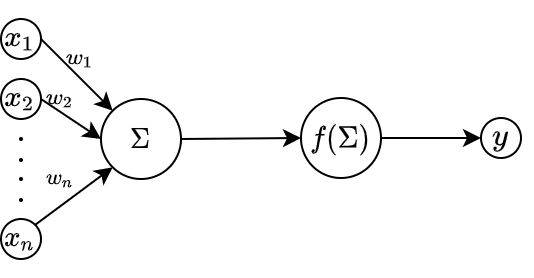
\includegraphics[width=0.5\textwidth]{imgs/perceptron.png}
    \label{fig:perceptron}
    \caption{Principle of a Perceptron}
    \end{center}
\end{figure}

\noindent For the activation function several different options are possible, among them are the Threshold/Heaviside-, linear-, sigmoid-, tanh- and RELU-functions. The pictures below show the five functions:

\begin{figure}[ht]
    \begin{center}
    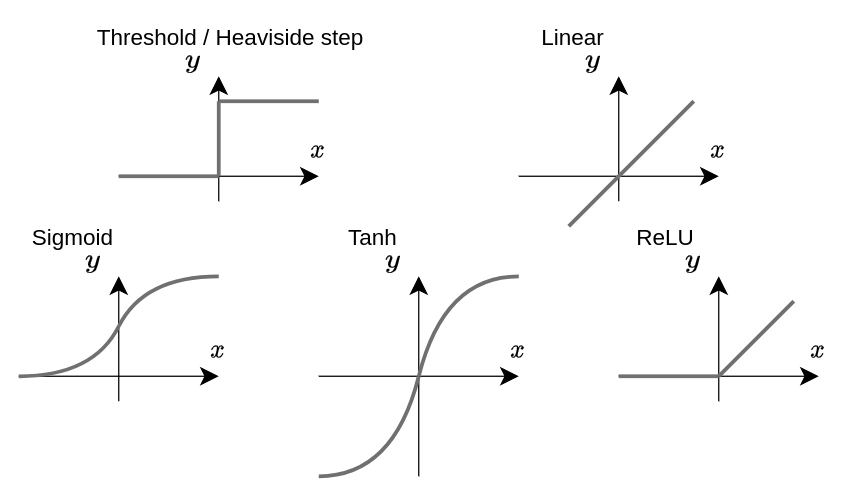
\includegraphics[width=0.5\textwidth]{imgs/perceptron_af.png}
    \label{fig:perceptron_af_0}
    \caption{Activation function 0}
    \end{center}
\end{figure}

\noindent Learning is achieved by repeatedly taking observations (from the training set) into account, then compute the output for each observation and check if it matches the correct output. I.e. one checks \(y = y'\), where \(y\) is the prediction and \(y'\) the true value.\\
Then one can update the weights of the perceptron according to the learning function. One can derive this learning function by computing the gradient. For this we must first define the loss, which is \(L = y' - y\). Then we take the squared loss and build the derivative to each \(w_i\):

\[\frac{\partial L^2}{\partial w_i} = 2 \cdot L \cdot f'(\sum_{j = 1}^n w_j \cdot x_j) \cdot x_i\]

\noindent This is now used to update the weight-values, for this one changes the \(2\) to the \textit{learning-rate-parameter} \(\alpha\):

\[w_i = w_i + \alpha \cdot L \cdot f'(\sum_{j = 1}^n w_j \cdot x_j) \cdot x_i\]

\noindent A perceptron can only linearly seperate data, therefore it can learn an \(and\)- or \(or\)-Gate, but not a XOR-Gate. Further if the data is messy, such that it is not linearly seperable it can also not learn it, but will \textit{oscilate} - therefore another stopping criteria is needed.

\subsubsection{Decision Trees}
\label{subsubsection:dt}


\noindent Decision Trees (DTs) are a rather old model, which can be depicted as a tree, where the inner nodes are decision nodes and the leaf nodes the classes.\\
They can either be constructed by experts or learned from data. The two easiest models of a Decision Tree are the \textit{1R (One Rule; Decision Stump)} tree and the \textit{ZeroR (Zero Rule)} trees. The first has just one rule, whereas the second one always returns the majority class. This is useful for a baseline classifier, i.e. DummyClassifier.\\
The \textbf{basic algorithm for the decision tree learning} goes repeatedly through all remaining features and selects the one where splitting seems to be the best. After the split this is done until all observations are predicted correctly, or if this is not possible one must result to other means. These other means consist normally of applying the majority function, but also a random draw is possible, etc...; To compute the ''best'' splitting measures 4 measures are presented in the lecture:

\begin{itemize}
    \item Error Rate: Goal is to minimize error rate. I.e. we look at all possible splits and take the one which is best, then repeat. One can use as the error rate for instance \(1 - acc_{micro}\), or \(1 - acc_{macro}\).
    \item Information Gain: For this a few more terms have to be introduced:
        \begin{itemize}
            \item \(l\) represents the amount of different classes (i.e. for eye-colors ''white'', ''pink'' and ''black'' \(l = 3\)).
            \item Entropy: \(H(X) = - \sum_{i = 1}^l p(x_i) \cdot log_2 \; p(x_i)\)
            \item Entropy measures the impurity of a feature and is \(1\) for a completely impure feature (e.g. \(50\%\) class 1 and \(50\%\) class 2) and \(0\) for a feature, where all values are the same.
            \item The goal is now to reduce entropy, which can be done by Information Gain (IG). It is calculated between the difference of the current entropy value and the sum of the relative entropies of the new splits (See next point).
            \item \(IG(X_1,...,X_j,...X_k) = H(X) - \sum_{i = 1}^k p(X_i) \cdot H(X_i)\)
        \end{itemize}
    \item Gini Impurity (Gini index)
        \begin{itemize}
            \item \(l\) represents the amount of different classes (i.e. for eye-colors ''white'', ''pink'' and ''black'' \(l = 3\)).
            \item Measures inequality between values of a distribution.
            \item ''How often a randomly chosen element from the set would be incorrectly labeled, if it was randomly labeled according to the distribution of labels in the subset''
            \item \(IG(p) = \sum_{i = 1}^l p_i (1 - p_i)\)
        \end{itemize}
    \item Relative Information Gain
        \begin{itemize}
            \item For this measure it is assumed, that one has already computed the Information-Gain \(IG\).
            \item The problem with the information gain is, that if one has a feature with very many different attributes like ID, then this feature would result in a perfect information gain and will always be selected. But this leads to a massive overfit, therefore the \textit{Relative Information Gain (IGR)} is introduced. For this the \textit{Split-Information-Gain (V)} is calculated.
            \item \(l\) represents the amount of different classes (i.e. for eye-colors ''white'', ''pink'' and ''black'' \(l = 3\)).
            \item \(V(X_1,...,X_j,...X_k) = - \sum_{i=1}^k \frac{|X_i|}{|X|} \cdot log_2 \;  \frac{|X_i|}{|X|}\)
            \item \(IGR(X_1,...,X_j,...X_k) = \frac{IG(X_1,...,X_j,...X_k)}{V(X_1,...,X_j,...X_k)}\)
        \end{itemize}
\end{itemize}

\noindent A problem for the above sketched learning algorithm is, that it could massively overfit the data. A method to combat this is \textit{(post-)pruning}, which removes parts of the tree by replacing the decision node with a majority vote. Also \textit{pre-pruning} is possible, which is done before/during the construction of the tree.\\
A further problem with decision trees is, that there stability is questionable at best, i.e. small changes in the training data may lead to significantly different datasets.

\subsubsection{Random Forests}

\noindent Is a combination of \textit{Boostrapping} (see \ref{subsubsec:bootstrapping}) and \textit{Decision Trees} (see \ref{subsubsection:dt}).\\
The basic idea is, that

\begin{enumerate}
    \item one first creates multiple datasets by making bootstrap samples
    \item then constructs for each such sample a decision tree
    \item and finally combines the decision trees in a certain way (e.g. Majority-Voting). 
\end{enumerate}

\noindent This works, as the decision trees are highly unstable and therefore small deviations in the training set, may lead to significantly different decision trees.\\
For evaluation one can use the default methods, but one additional is proposed:\\[1em]
\textbf{Out-of-bag error (OOB)}: As we use bootstrapping, it is likely that for a single bootstrap-sample not all observations from the original dataset are present. Therefore one can add the missing observations into a \textit{bag}. Then one evaluates the entries of the bag.\\
This process is now applied to each bootstrap sample, then one computes the average error of the observation and finally aggregates over all bootstrap samples.\\[1em]
The exact calculation should be the following, where \(N\) is the set of observations, \(B\) the set of bootstrap samples, function \(in(i,j)\) returns true iff observation \(i\) is contained in bag \(j\), \(value(i,j)\) is either 0 (if \(i\) is wrongly predicted) or 1 (if \(i\) is correctly predicted) and \(decisionFunction(oob_i)\) can be implemented in various ways, basically it needs to aggregate all predictions of the observation, which can for instance be done with a majority vote function or a mean calculation.\\
Note that in the lecture the Out-of-bar error is defined twice, although the defnitions are similar they differ in the details - the other one calculates the average out of bag error per bag, and then averages again (second algorithm).

\begin{lstlisting}[escapeinside={(*}{*)}]
(*\(oob\)*)... List of observations

for i in N:
    (*\(oob_i \leftarrow []\)*)
    for j in B:
        if in(i,j):
            (*\(oob_i.append(value(i,j))\)*)

    (*\(oob_i \leftarrow decisionFunction(oob_i)\)*)

(*\(oob_{value} \leftarrow \frac{\sum_{i \in N} oob_i}{|N|}\)*)
    
return (*\(oob_{value}\)*)

\end{lstlisting}


\begin{lstlisting}[escapeinside={(*}{*)}]
(*\(oob\)*)... List of observations

for i in B:
    (*\(oob_i \leftarrow []\)*)
    for j in i: (for each element in the bag)
        (*\(oob_i.append(value(j,i))\)*)

    (*\(oob_i \leftarrow \frac{\sum_{j \in i} oob_i[j]}{|i|}\)*)

(*\(oob_{value} \leftarrow \frac{\sum_{i \in B} oob_i}{|N|}\)*)
    
return (*\(oob_{value}\)*)

\end{lstlisting}



\subsubsection{Naive Bayes}
\label{subsubsec:naive-bayes}

\noindent Is a form of simple statistical modelling, which assumes:

\begin{itemize}
    \item All attributes are equally important
    \item All attributes are statistically independent (this actually doesn't hold most of the time)
\end{itemize}

\noindent We can now state the question, what is the probability of the class given an instance, where evidence \(E\) are the observations non-class attribute values and event \(H\) is the \textbf{class} value.\\
Bayes theorem tells us, that the \textit{posteriori} probability \(P(H|E)\), given the \textit{a priori} probability \(P(H)\), the \textit{likelihood} \(P(E|H)\) and the \textit{marginal} probability \(P(E)\) is:

\[P(H|E) = \frac{P(E|H) \cdot P(H)}{P(E)}\]

\noindent As we assume that the attributes (We have \(n\), the set of all attributes is denoted as \(N\)), are independent, we can take use of the product rule:

\[P(H|E) = \frac{P(E_1 | H) \cdot P(E_2 | H) \cdot ... \cdot P(E_n | H) \cdot P(H)}{P(E)} = \frac{P(H) \cdot \Pi_{i \in N} P(E_i | H)}{P(E)}\]

\noindent For this we can state, that we actually do not need the \textit{marginal} probability (\(P(E)\)), as this value is constant for the given \(E\), which normalizes the result to obtain a probability, but a likelihood is also fine for our purposes. This leaves us with (\(\propto\) means proportional):

\[P(H|E) \propto P(H) \cdot \Pi_{i \in N} P(E_i | H)\]

\noindent The goal of Naive Bayes can now be reduced to finding class \(c\) which maximizes the above equation, so:

\[p = \argmax_{c \in H} P(H = c) \Pi_{i \in N} P(E_i | H = c)\]

\noindent If the probability of a single \(P(E_i | H)\) is zero, than the posteriori will also be zero, which can be seen as a problem. Therefore the \textit{laplace estimator/correction/smoothing} exists, which is for a given probability calculation, where \(|N|\) is the total amount of samples, \(n_i\) the amount for \(i\), \(\alpha\) is the laplace correction value and \(d\) is the amount of different \(i's\) (i.e. for an attribute with 3 different classes it is \(d = 3\)):

\[\theta = \frac{n_i + \frac{\alpha}{d}}{|N|}\]


\noindent The next question arises, when one wants to take numeric attributes into account: How to do this?\\
To fix this problem, normally a \textit{Gaussian} probability distribution of the values are assumed:

\[\overline{x} = \frac{1}{|N|} \sum_{i \in N} x_i\]
\[s = \sqrt{\frac{1}{|N|-1} \sum_{i \in N} (x_i - \overline{x})^2}\]
\[f(x) = \frac{1}{\sqrt{2 \pi} \cdot s} e^{-\frac{1}{2} \cdot \left( \frac{x - \overline{x}}{s} \right)^2}\]

\noindent As probability densities are not probabilies, one must integrate them to gain them. But in principle after the transformation it works similar to the qualitative data approach we had above.

\subsubsection{Covering Algorithms}

\noindent At each step of the algorithm a rule is identified that ''covers'' some of the instances. Is somehow similar to a Decision Tree in the sense that it is basically a set of rules. The difference is most obvious in the multiclass case, where the covering algorithm focuses on a single class (i.e. generates all rules for the one class), where the decision tree takes all classes at the same time into account.\\
Covering algorithms work, that they add tests to the rule that is currently constructed. In contrast to this, decision trees work by adding tests to the tree that is under construction.\\
The goal is now to select a test, which maximizes accuracy. For this \(t\) denotes the number of instances covered by the rule, \(p\) the number of positive instances covered by the rule, \(t-p\) are the errors made by the rule, therefore one strives to maximize \(\frac{p}{t}\). We are finished when \(\frac{p}{t} = 1\).\\
In the lecture the pseudocode for \textit{PRISM} is provided, which basically works according to the above pricinple, by starting at one class and do the rule generation according to the \(\frac{p}{t}\) maximization mechanism. Then it adds such rules, until all instances with the class are identified correctly. Then it moves on to the next class, etc., etc.

\subsubsection{Bayesian Networks for Classification}

\noindent Although in the lecture Bayesian Networks are studied generally and therefore not with a focus on classification, in the following it is still regarded as to be contained in the classifier section. Before reading this section, be sure to read Section \ref{subsubsec:naive-bayes}.\\
A Bayesian Network consists of a set of variables (nodes), a set of directed arcs between the variables, together the nodes and arcs form a acyclic graph and the probabilities for every node given its parents is known.\\[1em]
As in the Naive Bayes, given evidence \(E\) one can select the class with the highest probability given \(E\), i.e. \(\argmax_{c \in H} P(H = c | E)\). In the Naive Bayes case we applied the product rule and discarded the marginal probability to obtain an easier to compute solution.\\
In the Bayesian Network case one can use the structure of the network to ease computation, i.e. that the probabilities for every node given its parents is known, therefore we only need to consider the part of the evidence \(E\) which is part of the parents of node \(H\).

\begin{figure}[ht]
    \begin{center}
    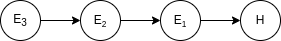
\includegraphics[width=0.5\textwidth]{imgs/bayesian-network.png}
    \caption{A Bayesian Network}
    \label{fig:bayesian-network}
    \end{center}
\end{figure}

Generally the computation of a joint probability, e.g. \(P(H = a, E_1 = t, E_2 = f)\), can be computed by the joint probability distribution. For example, consider the Bayesian Network depicted in figure \ref{fig:bayesian-network}. To calculate the Joint Probability Distribution given our example, we get:

\[P(H = a, E_1 = t, E_2 = t) = \sum_{e_3 \in E_3} P(H = a | E_1 = t) \cdot P(E_1 = t | E_2 = t) \cdot P(E_2 = t | E_3 = e_3) \cdot P(E_3 = e_3) \]

\noindent Note that \(P(H = a | E_1 = t)\) and \(P(E_1 = t | E_2 = t)\) are constant.\\
An algorithm for efficiently calculating the joint probability distribution is the \textit{Variable Eliminiation Algorithm}. Given a complete joint probability calculation with many sums, it takes out constant paths, that some parts don't need to be calculated again. Finding the best order is NP-hard, therfore usually heuristics are used for this process.\\[1em]
\textbf{D-Seperation}: To check whether two variables are independent given some evidence (I think this is useful to speed up computation of the joint probabilities), one can use D-Seperation. In general in D-Seperation one must distinguish between three types of Node-Structures (See Figure \ref{fig:d-sep} and the three points below):

\begin{figure}[ht]
    \begin{center}
    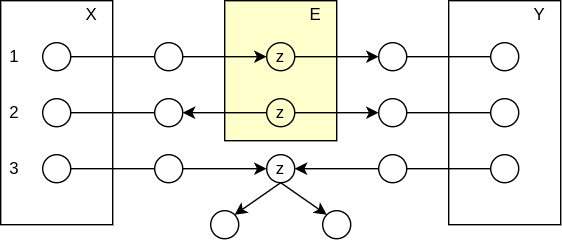
\includegraphics[width=0.5\textwidth]{imgs/d-sep.png}
    \caption{D-Seperation}
    \label{fig:d-sep}
    \end{center}
\end{figure}

\begin{enumerate}
    \item Is called a seriel connection. \(X\) and \(Y\) are seperated given that \(z\) is in the evidence \(E\).
    \item Is called diverging connection. \(X\) and \(Y\) are seperated given that \(z\) is in the evidence \(E\).
    \item Is called converging connection. \(X\) and \(Y\) are seperated, if \(z\) is NOT in the evidence \(E\) and further no descendent of \(z\) is in \(E\).
\end{enumerate}

\noindent The next question to answer regarding Bayesian Networks is how to construct these things?\\
In general two options are possible: Experts construct it, or it is learned from the data. Further it can be stated that human experts are better in finding the structure of the network, whereas machines are better for calculating the probabilities.\\
Given a network one can calculate the probabilites by counting, e.g. for calculating the probability \(P(H = t | E_1 = t)\) one counts \(\#(H = t \land E_1 = t)\) and divides this by \(\#(E_1 = t)\). The other probabilities can be calculated accordingly.\\
Learning the structure is harder. As a measurement for how good the model fits the data, the \textit{goodness of fit} measure is introduced, where \(D\) denotes the data set and \(M\) denotes the model, \(j\) denotes an individual observation and \(i\) denotes the attributes/nodes:

\[P(D|M) = \Pi_j P(s^j | M) = \Pi_j \Pi_i P(N_i = v_i^j | Parents(N_i), M)\]

\noindent Further the log likelihood is introduced:

\[log P(D|M) = \sum_j \sum_i P(N_i = v_i^j | Parents(N_i), M)\]

\noindent A good model should have a good fit of the data and further should have a low complexity (not many parameters), so the objective should be to maximize (where \(\alpha\) is a parameter that controls how important it is to reduce the complexity of the network and \(\#M\) denotes the amount of parameters):

\[log P(D|M) - \alpha \#M\]

\noindent With this performance measure in mind, one can construct search algorithms for finding the best structure. For instance one can use meta heurstics, like hill climbing, evolutionary algorithms, tabu search, simulated annealing, etc., etc..\\
For the hill climbing/local search method, one can use this five step process:
\begin{enumerate}
    \item Construct an initial network
    \item Calculate the score of the current BN network
    \item Generate the neighborhood by modifying the current network
    \item Select one of the networks in the neighborhood as a new current network for the next iteration
    \item Go to step 3 if termination criteria is not fulfilled
\end{enumerate}

\subsection{Support Vector Machines (SVMs)}

\noindent SVMs are a type of classifier, which try to seperate linear seperable data. They are intrinsically binary classifiers, i.e. can only classify between two classes. To extend them to multiclassification one can use for instance \(1\) vs \(all\) (Classify one class against all other classes, create a model for each class) classification.\\
SVMs are a method which try to seperate data in a ''best possible way''. In a basic mode they only seperate linear data. When one wants to perform non-linear classification, one can use the \textit{kernel trick}, to map the data into high dimensional feature space which is again linearly seperable.\\
The name of SVMs come from ''Support Vectors'', which are vectors in the data-space which seperate the data linearly (seperating line/margin line).\\[1em]
The lecture just gives a rough (but very mathematical) overview, therefore in the following a few key terms are listed and explaiend:

\begin{itemize}
    \item Hard-Margin: If the data is exactly linearly seperable, one can exactly classify the data
    \item Soft-Margin: If the data is not exactly linearly seperable, one can use a soft-margin to allow some observations to be misclassified
    \item Kernel: Is a mathematical function, which transform the data.
    \item Non-linear kernels: If the data is not linearly seperable, then it might be in a higher-dimension.
\end{itemize}

\noindent In general SVMs seem to be good for rather small datasets and SVMs are not always better. Further it is noted, that kernels can also be used with other algorithms and not only SVMs.\\
As far as the literature shows, an SVM always finds the \textit{optimal hyperplane} by e.g. Lagrange Optimization (\url{https://web.mit.edu/6.034/wwwbob/svm-notes-long-08.pdf}).


\newpage
\section{Regression}

\noindent Regression is all about predicting numeric values, e.g. house prices.\\

\subsection{Performance Measures}

\noindent Compared to Classification other performance measures must be used, in the following a few of them are presented:

\begin{itemize}
    \item \textbf{Mean Squared Error (MSE)}:
        \begin{itemize}
            \item When we have \(n\) samples, the MSE is calculated by taking the mean of the squared differences between the predicted \(\hat(Y_i)\) and the observed (aka. true) \(Y_i\) values.
            \item \(MSE = \frac{1}{n} \cdot \sum_{i = 1}^n (Y_i - \hat{Y_i})^2\)
        \end{itemize}
    \item \textbf{Root Mean Squared Error (RMSE)}:
        \begin{itemize}
            \item \(RMSE = \sqrt{MSE}\)
        \end{itemize}
    \item \textbf{Mean Absolute Error (MAE)}:
        \begin{itemize}
            \item Given \(n\) samples, the MAE is calculated by averaging the absolute errors.
            \item \(MAE = \frac{1}{n} \cdot \sum_{i = 1}^n |Y_i - \hat{Y_i}|\)
        \end{itemize}
    \item \textbf{Median Absolute Error (MAD)}:
        \begin{itemize}
            \item Given \(n\) samples, the MAD is calculated by taking the median of the absolute errors.
            \item \(MAD = median(|Y_1 - \hat{Y_1}|, ... , |Y_n - \hat{Y_n}|)\)
        \end{itemize}
    \item \textbf{\(R^2\)-Score}:
        \begin{itemize}
            \item Is a measure for the goodness of fit.
            \item Has a range of theoretically \((-\infty, 1]\), where \(1\) represents the best value.
            \item In SciKit-Learn it is defined as (note, \(\hat{Y_i}\) denotes the prediction and \(\overline{Y_i}\) denotes the mean of the observed/true values):
            \item \(R^2 = 1 - \frac{u}{v} = 1 - \frac{\sum_{i = 1}^n (Y_i - \hat{Y_i})^2}{\sum_{i = 1}^n (Y_i - \overline{Y_i})^2}\)
        \end{itemize}
\end{itemize}

\subsection{Models}

\noindent Many of the models described in section \ref{subsec:class-models} can be transformed into a regression task, further a few new ones are introduced. All of the following are discussed in the lecture:

\subsubsection{Linear Regression}

\noindent Is the task of fitting a line \(y = w_0 + \sum_{j = 1}^l w_j \cdot x_j\), where \(l\) denotes the dimensions to predict. The task is then to calculate the best values for \(w_j\), for which one must at first define a cost metric which should be minimized. This cost metric is the \textit{Residual Sum of Squared (RSS)}:

\[RSS(w) = \sum_{i = 1}^n (y_i - (w_0 + \sum_{j = 1}^l w_j \cdot x_{ij}))^2\]

\noindent The solution to this minimization problem can either be found in an analytical way or by an iterative algorithm, the gradient descent algorith, which basically works by calculating the gradient and moving along the gradient to a better solution (basically the same for the Perceptron in \ref{subsubsec:perceptron}, here again \(\alpha\) denotes the learning rate):

\[w_j = w_j - \alpha \frac{\partial RSS(w)}{\partial w_j} \]

\noindent This update is performed until convergence, where all \(w_j\) are updated simultaneously. Further an analytical approach exists, which is shown below how one may derive it. For this one takes the RSS, then does a bit of Matrix magic (just transformations) and then takes the derivative. After taking the derivative the resulting part is set to zero (strongest gradient) and one has the analytical approach: 

\[RSS(w) = \sum_{i = 1}^n (y_i - (w_0 + \sum_{j = 1}^l w_j \cdot x_{ij}))^2\]
\[= (\mathbf{y} - \mathbf{Xw})^T (\mathbf{y} - \mathbf{Xw})\]
\[= \mathbf{y}^T \mathbf{y} - 2 w^T \mathbf{X}^T \mathbf{y} + w^T \mathbf{X}^T \mathbf{X} w\]
\[\frac{\partial RSS(w)}{\partial w} = 0 - 2 \mathbf{X}^T \mathbf{y} + 2 \mathbf{X}^T \mathbf{X} w\]
\[w = (\mathbf{X}^T \mathbf{X})^{-1} \mathbf{X}^T \mathbf{y} \]

\subsubsection{Other regression techniques}

\noindent Other regression techniques exist, like polynomial-, ridge- and lasso-regression.\\
\textbf{Polynomial} regression strives to fit data, which is better predicted by a non linear approach.\\[1em]
\textbf{Ridge} and \textbf{Lasso} regression both want the same things: Minimize the amount of needed variables which should therefore prevent overfitting. They do this by adding an additional term to the cost function (where \(||w||_2^2\) is normally the euclidean norm (in the lecture the square root is not taken) and the \(||w||_1\) is normally the manhatten distance):

\[Cost_{Ridge} = RSS(w) + \lambda \cdot ||w||_2^2\]
\[Cost_{Lasso} = RSS(w) + \lambda \cdot ||w||_1\]

\subsubsection{KNN-Regression}

\noindent Similar to normal KNN, so first calculating nearest neighbors, but then instead of taking the majority vote for the class, one can calculate the mean among the nearest points - done. E.g. for a \(k=5\) KNN:

\[y_i = \frac{\sum_{j \in NearestFive(x_i)} \hat{y}_j}{5}\]

\subsubsection{Regression- and Model-Trees}

\noindent Similar to decision trees, but the splitting criterion is different (minimizes intra-subset variation), the termination criterion is different (standard deviation becomes small enough), the pruning criterion is different (based on numeric error measure) and the prediction is different (predicts average value of instances). To predict a certain value, one traverses through the tree, then goes to the leaf node and looks up the value there.\\
More sophisticated method is the Model-Tree, which has for each leaf node a linear-regression function.

\newpage
\section{Reinforcement Learning (RL)}

\noindent Is a type of learning that is inspired from nature (trial and error learning), e.g. one does not touch a hot place twice (except one is a scientist). It is different from supervised learning, as in RL must make sense of the world from it's own experience, where an agent quickly comes into the exploration/exploitation dilema, which means that an agent wants to take the best possible action, but an agent can only take this action when it knows that this action is the best and for this exploration is necessary.\\

\subsection{Components of a RL system}

For RL to work out several things are necessary:
\begin{itemize}
    \item Policy/Action - Selects an action which an agent should take, e.g. Selecting a slot machine in a casino
    \item Reward Signal - Immediate reward from the environment, e.g. Reward from the slot machine.
    \item Value Function - What the agent thinks, a policy is worth, e.g. The agent thinks, that slot machine B is best.
    \item Model/State (Optional) - Model of the environment 
\end{itemize}

\noindent The lecture presents a few tabular solution methods, where \textit{tabular} just means, that state and action spaces are small and that they can be saved in a table.\\

\subsection{Action selection methods}

\noindent Different possible, in the lecture:

\begin{itemize}
    \item Greedy action selection: Always take the best, i.e. \(A_t = \argmax_a Q_t(a)\)
    \item \(\epsilon\)-Greedy action selection: With probability \(1 - \epsilon\): Make greedy selection. With probability \(\epsilon\) make a random draw.
    \item Roulette wheel selection: Create a probability function where better actions have a higher probability of selection and make a random draw from this probability function.
    \item And they also provide the \textit{Upper-Confidence-Bound Action Selection} mechanism, which works like: \(A_t = \argmax_a \left[ Q_t(a) + c \sqrt{\frac{ln t}{N_t(a)}} \right] \)
\end{itemize}

\subsection{Multi Armed Bandit (MAB)}

\noindent Several possible options for actions possible, task is to select the best one. We do not have a state. And the goal can be defined mathematically as (\(q_*(a)\) is the true probability/value of action a, \(E\) is the expectation, \(R_t\) is the reward, \(A_t = a\) is the selected action \(a\)):

\[q_*(a) = E[R_t | A_t = a]\]

\noindent So the goal of the MAB is to model \(Q(a)\) as close as possible to \(q_*(a)\).\\
The basic update of the values can be defined as (\(1_{A_i = a}\) is 1 if \(a\) was selected at time \(t\), otherwise 0):

\[Q_t(a) = \frac{sum \; of \; rewards \; when \; a \; taken \; prior \; to \; t}{number \; of \; times \; a \; taken \; prior \; to \; t} = \frac{\sum_{i = 1}^{t-1} R_i \cdot 1_{A_i = a}}{\sum_{i = 1}^{t-1} 1_{A_i = a}}\]

\noindent The above formula has one significant downside: It cannot be computed \textit{on-the-fly/online}, i.e. it must be computed with all previous values after each update. Therefore the lecture also provides an incremental version of the above value estimation.\\
Further it provides an update for non stationary problems, i.e. where \(q_*(a)\) changes over time. They fix this by using the incremental version but give more recent values a higher priority.\\
Another evaluation method is, that at the beginning one does not initialize the \(Q(a)\) with 0, but takes an optimistic approach.\\

\subsection{Markov Decision Process (MDP)}

\noindent As in MABs we have feedback, but now also states/a model of the environment. The basic difference for action selection and value updates is, that one now selects the best action per time-state tuple and also updates the value per time-state tuple, not just per time.\\[1em]
In this context also the \textit{Bellman Equation} is mentioned, which expresses a relationship between the value of a state and the values of its successor states. The bellman equation can be computed by dynamic programming.\\[1em]
Further \textit{Monte Carlo Methods} exist, which sample sequences and then learn from the sequences.\\[1em]
The last topic in the lecture is \textit{Temporal-Difference learning}, which is a central idea of reinforcement learning. They can learn directly from experience without a model. They operate as Monte Carlo Methods on episodes, but learn after each time step. \textit{Q-Learning} is a very popular Temporal-Difference algorithm.


\newpage
\section{Feature-Selection, Auto-ML, Hyper-Parameter-Tuning, Ensemble Learning and similar things}

\subsection{Feature Selection}

\noindent One should select features that minimize redundancy and maximize the relevance to the target. This means, that for say 10 attributes in a given dataset, one wants to select those, which seem to be the most informative.\\
A naive approach is to tryout all subsets of the 10 features, which results in \(2^{10}\) possibilities - which is infeasible, for a large amount of attributes, therefore the task of features selection is NP-hard.\\[1em]
One can use search to find a local optimum of features to use, by e.g. using a genetic algorithm. Other strategies are for instance using a greedy approach, which comes in two flavors: \textit{Forward Selection} starts with an empty set of features, then features are added iteratively by comparing how good they improve the performance measure, until the desired number of features is selected.\\
\textit{Backward elimination} starts with all features selected and eliminates all those features iteratively, which seem to not contribute to the current performance of the model, until we arrive at the desired number of features.\\[1em]
Other possibilities for feature selection include dimensionality reductions, such as the Principal Component Analysis (PCA), Analysis of Correlation or Factor Analysis.\\
Again other (supervised) methods exist, like entropy/information gain, mutual information, maximum likelihood estimation, odds ration,...\\[1em]
Two further methods are presented, a wrapper (using the algorithm as a performance measure, by using search strategies) and a filter (using another proxy measure, a lot faster...) strategy.\\


\subsection{Meta Learning}

\noindent Can be described with \textit{Learning about learning} and deals with many machine learning techniques, like model selection, method combination or Hyper-Parameter-Tuning.\\
To begin, one must know the \textit{No Fre Lunch (NFL)} theorem, which states that ''any two algorithms are equivalent when their performance is averaged across all possible problems'' (\cite{nfl}) .\\[1em]

\subsubsection{Algorithm/Model Selection}


The first problem discussed is the one of \textit{Algorithm Selection}, where it is hard to evaluate the performance of an algorithm, because taking the NFL theorem into account it is hard where should it be evaluated: On a single problem?, or on a certain set of problems? or on something entirely different?\\
The lecture provides two possibilities for possible performance measurements:
\begin{itemize}
    \item Closed Classification World Assumption (CCWA)
    \begin{itemize}
        \item Assume that the problems the algorithm works on, are a certain subset of real life problems.
        \item Therefore one can show, that the algorithm works better on this subset.
        \item Is favored, as therefore one can easily compare algorithms, but in practice it is sometimes hard to characterize real-life classification tasks.
    \end{itemize}
    \item Open Classification World Assumption (OCWA)
    \begin{itemize}
        \item Assume that there is no such structure.
        \item Class of tasks, in which algorithm performs well is characterized.
    \end{itemize}
\end{itemize}

\noindent An example for a detailed formulation of a CCWA is the Rice Framework (see Figure \ref{fig:rice-framework}), which is formulated like \textit{For a given problem instance \(x \in P\), with features \(f(x) \in F\), find the selection mapping \(S(f(x))\) into algorithm space \(A\), such that the selected algorithm \(\alpha \in A\) maximizes the performance mapping \(y(\alpha(x)) \in Y\).}\\
This basically means, that we want to learn \(S\) (the selection mapping), which is just a fancy term for associating a problem with an algorithm (finding the best algorithm \(\alpha\) for problem \(x\)).\\


\begin{figure}[ht]
    \begin{center}
    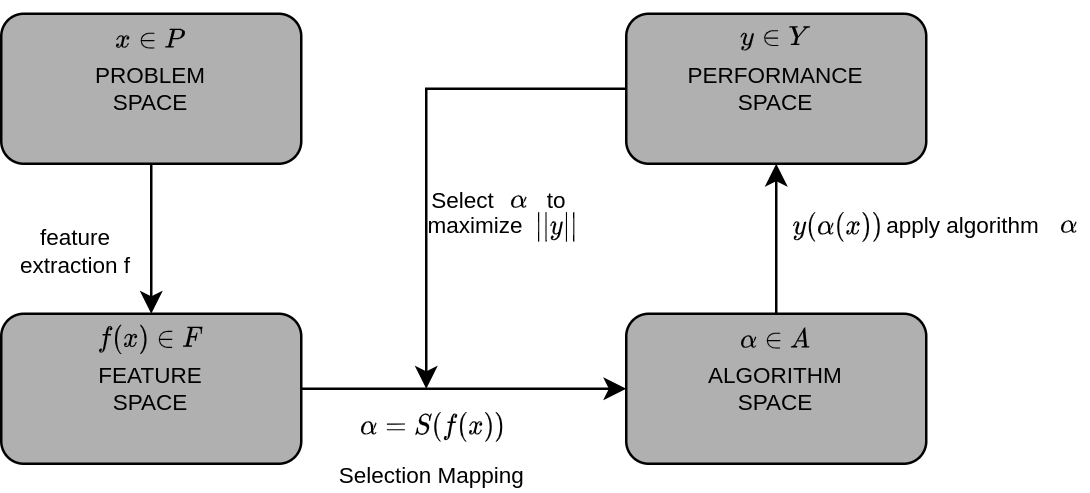
\includegraphics[width=0.5\textwidth]{imgs/rice-framework.png}
    \caption{Rice-Framework}
    \label{fig:rice-framework}
    \end{center}
\end{figure}

\noindent In Meta Learning it is very important to select the right features for a given problem, for instance one can use Statistical-/Information-theoretic-(like \textit{Number of Attributes}, \textit{Number of classes}, \textit{Some ratios}, \textit{Averages}), Model-based- (like for a decision tree the properties of it (maximum tree depth,...)), Landmarking- (see below) or Computational-cost-features.\\
\textit{Landmarking} is a process which takes algorithms and checks on which problems the algorithms work well (these algorithms are called \textit{Landmarker}s). With the performances of these Landmarkers on certain problems, one can state something about the nature of these problems.\\
Further and important for algorithm selection, these landmarkers should be highly efficient in terms of performance, so they should be fast. Also one should be able to associate an algorithm with landmarkers, e.g. for algorithm a1, the landmarkers i1 and i2 correspond roughly to the problems, on which it works well.\\

\subsubsection{Hyper-Parameter Optimization (HPO)}

\noindent HPO is an important topic for tweeking machine learning models. It can be described as a search problem, therefore normal metaheuristics, etc. can be used for it.\\
The easiest techniques to use are Grid- and Random-search. Grid search is an exhaustive search, which just searches all different possibilities in a well defined multi-dimensional-grid.\\
Randomized search selects a few random hyper-parameters and checks their performance.\\[1em]
A very promising technique is \textit{Sequential Model-based Bayesian Optimization}. It is a general framework for minimizing blackbox functions \textit{f}. As the name suggests it uses bayes as the baseline for it's optimization, so remember:

\[P(H|E) = \frac{P(E|H) \cdot P(H)}{P(E)}\]

\noindent As we are again not interested in the specific probability we can drop \(P(E)\) as in Naive-Bayes (\(\propto\) means proportional):

\[P(H|E) \propto  P(E|H) \cdot P(H)\]

\noindent The bayesian optimization process now assumes a probability distribution \(P(H)\), which model ''how well certain Hyper-Parameters work'', i.e. the higher the better. At the beginning of the Bayesian-Optimization process this must not be the ''true'' value, therefore it iteratively it's prediction by computing the posterior \(P(H|E)\), by taking into account new evidence \(E\) which was sampled from the true function.\\
The function that approximates the true \(P(H)\) is called \textbf{Surrogate Function} and should be efficient. The function which selects the best algorithm selection from the surrogate function is called \textbf{Acquisition Function}.
A pretty good explanation can be found in: \url{https://machinelearningmastery.com/what-is-bayesian-optimization/}

\subsubsection{AutoML}

\noindent Combines several things like \textit{Feature Selection}, \textit{Feature Preprocessing}, \textit{Feature Construction}, \textit{Model Selection} and \textit{Parameter Optimization}.

\subsection{Ensemble Learning}

\noindent Ensemble Learning can be seen as a sort of learning, which combines several classifiers to improve performance of the overall model. An example for this is the Random Forest classifier, which combines serveral Decision Trees.\\
The terminology for ensemble learning is quite clearly defined: There exist Homogenous (i.e. all classifiers are of the same type) and Heterogeneous (i.e. classifiers may differ) ensemble learning techniques. Random Forests are homogeneous, as they only use Decision Trees.\\
One can combine the classifiers by majority voting, i.e. selecting the class which most classifiers predict. For this it is important to note, that a classifier may have different types of output:
\begin{enumerate}
    \item Type 1 - Abstract Level: Classifier produces only the class/label prediction
    \item Type 2 - Rank Level: Classifier produces a list of probable class labels 
    \item Type 3 - Measurement Level: Classifier procudes probability distribution for each labels.
\end{enumerate}

\noindent Depending what the output of the classifiers are, the ensemble decision maker may make decisions not only on majority voting, but e.g. maximizing the probabilites, or averaging them.\\
When using majority voting, one can estimate the accuracy of the ensemlbe when one assumes independence between the classifiers and all classifiers have equal accuracy:

\[P_{maj} = \sum_{m = |L/2| + 1}^L \binom{L}{m} p^m (1 - p)^{L - m} \]

\noindent This would in theory lead to the conclusion, that one may just add an infinite amount of classifiers and gain \(100\%\) accuracy, but this does not work in real life... I think the reason for this is, that the classifiers may fail on the same observations, as the observations are inherently hard to predict.\\[1em]

\subsubsection{Bagging}

\noindent Tries to achieve independent classifiers by varying the training set, as it is done with Random Forests. I.e. one takes bootstrap samples from the data set.\\
For this to work out, the classifiers should be unstable and class decision vote is taken by plurality vote.

\subsubsection{Boosting}

\noindent Boosting is a process, where a classifier depends on a prdecessor. In the process the errors from the predecessor is analysed and decided which part of the data to focus on and weights are set for ''hard'' parts.\\
Initially the weights are \textbf{equal} amont all training samples, e.g. \(\frac{1}{n}\) for each observation.\\[1em]
The iterative process works as in the following: A sample is taken, and classifiers are trained. Then the weights are adjusted to give more importance to misclassified samples. Subsequent classifiers should thus focus on the hard samples by either directly utilizing weights in the learning algorithm or by sampling techniques which sample the hard parts multiple times.\\[1em]
\textbf{AdaBoost} is an iterative ensemble learning algorithm, which has a pool of classifiers \(h\) and a number of iterations \(T\). The final classifier is a linear combination of the individual classifiers, which are comprised of the classifiers \(h\) and a coefficient \(\alpha\):

\[H(x) = sign(f(x)) = sign (\sum_{t = 1}^T \alpha_t h_t(x))\]

\noindent When learning AdaBoost, it takes care of the values which were misclassified previously. The classifier coefficient is calculated by how good the classifier works on the current weighted data set.\\[1em]

\textbf{Gradient Boosting} is another boosting technique which combines gradient descent with boosting. Is again an iterative process, where in each stage a new weak learner is introduced to compensate the shortcomings of the previous weak learners. In Gradient Boosting the shortcomings are identified by gradients.






\newpage
\section{Multi-Layer Perceptrons and Deep-Learning}

\subsection{Multi-Layer Perceptrons (MLP)}

\noindent Combines several perceptrons into layers, where each layer is composed of perceptrons. MLPs are \textit{feed-forward} Neural Networks, which means, that they do not have cycles.\\
This means, that e.g. we have 5 neurons in the first layer, 3 in the second and 4 in the third. Generally the first layer is described as the \textbf{input} layer, the last layer as the \textbf{output} layer and all layers in between are called \textbf{hidden} layers.\\
Each neuron has the same structure as a perceptron, with an activation function, which were already discussed in the perceptron part (See Section \ref{subsubsec:perceptron}). For MLPs it mostly holds, that all neurons have the same activation function. Further it is noted that for some tasks, like multiclass-classification, it is necessary to give the output of the last layer as a probability distribution. This can be achieved by the \textbf{Softmax} layer/function. It scales all outputs to a probability distribution, i.e. all outputs some up to 1 and each single one is in the range \([0,1]\).\\[1em]
Learning is in principle for each neuron similar to perceptron learning, the difference is that now on cannot simply train all neurons at once. For this one starts at the output layer, trains each neuron, then moves one layer to the front. For this layer one must now first calculate the relative errors, which they receive from the layer further at the output. After this calculation one can now train them and then move one layer back. One can iteratively continue this process, until one reaches the input layer. This process is called \textbf{Backpropagation}.\\
A pretty good pseudocode algorithm for Backpropagation can be found in (\cite{aima}).\\[1em]
Further the lecture distinguishes between three different types of learning, for this one must know the concept of epochs. An epoch is one forward and one backpropagation pass over all of the provided training samples (\url{https://www.kaggle.com/code/residentmario/full-batch-mini-batch-and-online-learning/notebook}).\\

\begin{itemize}
    \item Full-Batch: Computes the true gradient of the epoch, by computing the gradient of each training case independently, then summing the resultant vectors together.
    \item Mini-Batch: One splits a single epoch into multiple batches and updates the weight values for each such batch.
    \item Stochastic-Gradient-Descent: After each single data instance, the weights are updated (is termed as Stochastic as this is not the true gradient of all the data in the epoch).
\end{itemize}

\noindent One further advanced topic is MLP-regularisation, which tries to prevent overfitting of models. Can be implemented similar to rdige/lasso regression (just adding additional cost).\\

\subsection{Deep-Learning}

\noindent So what is Deep Learning? There are several definitions, in general it is something that is associated with neural networks, more precisely Multi-Layer perceptrons (see previous Section), which is composed of several smaller ''learnable units/functions''. Therfore the learnable function (the Neural-Network as a whole) is a stack of many simpler functions, that often have the same form.\\
\noindent Exact definitions for Deep-Learning are hard to give, one such definition simply says, that there must be multiple (\(\geq 2\)) hidden-layers, which would also include very shallow networks.\\
According to the lecture such networks are not seen as ''deep'', they do not provide an exact definition, but just state that the network must have ''very many layers''.\\[1em]
The main reason for ''goind deep'' is, that they perform well on certain practical tasks, such as Image Recognition. In theory ''going deep'' is not necessary, as a neural network with just one hidden layer (and arbtitrarily many nodes) can learn any function, but it is much harder for such a shallow structure to find a suitable network. Finding a deep one is up to now a more pracitcal approach.\\
Still such network are inherently hard to train, therefore one tries to reuse certain aspects of other deep-networks, such as the \textbf{architecture} or even the \textbf{parameters} via \textbf{Transfer Learning}.\\[1em]
In contrast to classical-machine-learning, Deep-Learning features also learning of the relevant features, how to process them and generally feature extraction (See section \ref{subsec:feature-extraction}). A very often used class of networks for such a task is the class of \textit{Convolutional Networks}. They typically consist of three types of layers:\\

\begin{itemize}
    \item Convolutional Layer
        \begin{itemize}
            \item Basically applies filters to an image.
            \item Such filters are used for edge detection, sharpening, etc.
            \item As the convolutional layer is learned, the filters are also learned.
            \item In the lecture slided they provide a few typical filters.
            \item Further this layer handles things like rotation of images, sizes, etc.
        \end{itemize}
    \item Sub-Sampling Layer / Pooling step / Downsampling
        \begin{itemize}
            \item Reduces the size of feature maps (so condences the information)
        \end{itemize}
    \item Fully connected MLP
        \begin{itemize}
            \item Is a fully connected MLP
            \item Typically at the end of the Deep-Network, to provide classification.
        \end{itemize}
\end{itemize}

\noindent In the lecture they quickly go over the following CNN architectures: \textit{LeNet}, \textit{AlexNet}, \textit{ZFNet}, \textit{VGG Net}, \textit{GoogLeNet}, \textit{ResNet}, \textit{Densenet} and \textit{SqueezeNet}.\\
To think of a new functioning network is very time and resource intensive, therefore reusing other architectures is highly recommended. One such way to do it is called Transfer Learning, which takes part of a pre-trained network for a different domain, for a different source task and adapts the rest of it for your task at hand. One can do this by cutting off the top layer(s) of a network and replace these with a supervised objective for a certain target domain.\\
The bottom \(n\) layers can either be frozen (i.e. not updated at all, recommended if one has a scarce database) or fine-tuned (i.e. updated, recommended if one has many labels). This combination is often better in practice than specialized classifiers.\\
One can also try a similar approach on unlabeled data, where the task is to train a model on just unlabeled data. Here one can take a pretrained network, cut off the upper part and do unsupervised learning on top of it (like clustering).\\[1em]
Further it is noted that one can visualize how individual layers work. This is in the context of interpretable AI, so one can see what is going on in the layesr. Another topic is data augmentation, which is important in the training process, as it strives to prevent the network from learning irrelevant facts.\\
Lastly the lecture recommends to use the \textit{RELU} activation function, as for some other functions the problem of a \textit{weak gradient} can appear, e.g. take the Sigmoid function, if you look at it from a distance it looks like a heaviside function...\\
Another tip is to use dropout while learning, which is a technique that randomly removes a part of the neurons. And finally they discuss various alternative methods for the standard gradient-descent algorithm, with a focus of how to select the learning rate \(\alpha\). They present the \textit{Stochastic Gradient Descent with Momentum} algorithm, which ''builds up momentum'' if the gradients keep staying in the same direction. Analogy is a ball which rolls down a hill.\\[1em]


\subsection{Recurrent Neural Networks (RNN)}

\noindent Have cycles in their neural network structure, which means, that they can operate over sequences of data, like sound. Often they have a sort of state (memory) and further the input and output size is variable.\\
Can architecturally be seen as a combination of recurrent layers, where each recurrent layer processes an input together with their output. Learning is basically done via backpropagation.\\[1em]
Long Short-Term Memory (LSTM) can store longer term memory, where at each step the old value can be kept or updated to a new value.\\
Gated Recurrent Units (GRUs) have similar performance but fewer parameters than LSTM. Other architectures are for instance auto-encoders, etc. etc.


\newpage
\section{Advanced Topics in ML}

\subsection{Feature Extraction}
\label{subsec:feature-extraction}

\noindent The following techniques are for ''manual-feature-extraction'' and can be sometimes ommitted for Deep-Learning.

\subsubsection{Text}

\noindent For text one can extract features by analysing the data. The lecture presents the Bag-oF-Words technique, which is done in the following steps:

\begin{enumerate}
    \item Tokenization - Cut character sequence into word tokens (e.g. single word like ''car'' ord phrases like ''a state-of-the-art solution'')
    \item Normalization - Map text and query term to same form (e.g. U.S.A to USA)
    \item Stemming - Words with the same stem should sometimes be regarded as the same, e.g. ''authorize'', ''authorization''
    \item Stop words - Removal of ''unnecessary'' words like ''to'', ''a'',...
    \item Then one can create a bar-og-words, i.e. removing the original text column from the data and adding as many columns as there are token vectors.
\end{enumerate}


\subsubsection{Image}

\noindent Different techniques exist, like Edge detection, Corner detection, Scale-invariant feature transformation, filters Bag-of-visual-words.\\
For some of those things one can use a filter. A filter is represented as a filter-kernel, which is basically a matrix, which is then applied to the image via the mathematical process of folding.

\subsubsection{Audio}

\noindent Often a series of steps, which analyzes the data according to some transformations and spectrum analyzers.


\subsection{Robustness/Adversarial ML}

\noindent One of the current biggest problems for ML is it's robustness and the social/real-life implications of this. Take for example the Google-Photos bug, where Google-Photos classified a person of color as a Gorilla, which lead to an outcry.\\
Other attacks comprise of attacks on Image-Classification, such as when one fools a Image Classifier to predict a Coala as a Banana. Such attack are mostly \textit{Evasion Attacks}, which try to fool the prediction steps by providing minimal perturbations of the input to achieve other outputs. There are several methods, that try to combat this/exploit this. Sometimes it is only necessary to change a single pixel to obtain completely ridiculous classifications, like classifying a horse as a frog. But this can also be dangerous, e.g. when a self driving car classifies a stop shield as a 90 km/h shield...\\[1em]
Possible attacks for a ML model include:

\begin{itemize}
    \item Evasion attacks - Fool prediction steps, by minimal perturbations of the input
    \item Poisoning (Backdoor) attacks - Attack during the learning of the model, goal is to embed a specific pattern that can trigger the malicious behavior. Possible defense: Pruning the network, which might reduce accuracy but generalization may impŕove.
    \item Model inference/inversion - Determine if a person participated in a medical DB
    \item Model Extraction/Stealing - Attacker tries to learn model approximation in as few queries as possible
    \item Confidentiality attacks - Exposure of sensitive data
    \item Availability attacks - Disruption of critical service
    \item Integrity attacks - Unauthorized modification of data
\end{itemize}


\subsection{Explainability of AI}

\noindent Is currently a major research topic in AI, which tries to find out how to inform humans, how an AI arrived at it's decision. This is done via explanations, where it is inherently harder for some machine learning models than for others to explain something.\\
E.g. it is pretty straight forward for a decision tree to explain a certain decision, whereas for a Deep-Neural-Network it may not be the case.\\
The researchers in this field distinguish between three types of explainability:
\begin{itemize}
    \item \textit{Intrinsic}: Model-inherent (i.e. linear model or decision-tree)
    \item \textit{Post-Hoc}: Extracting information from the model
    \item \textit{Ex-ante}: Data statistics, bias in data, definition of task
\end{itemize}

\noindent And further different types of explanations are discussed:

\begin{itemize}
    \item Feature statistics/visualizations
    \item Model internals (e.g. weights)
    \item Examples and counter-examples
    \item Proxy models: simpler, easier to understand surrogate model
\end{itemize}

\noindent Further it is pointed out, that the quality of explanations is also important, e.g. things like generalizations, truthfulness and contrastiveness (not just ''why x?'' but also ''why x not y?'') are important.\\
In the end they compare the explainability of different models to each other (Decision Trees best, Deep learning worst).

\subsection{Privacy and AI}

\noindent As for AI large amounts of data are needed and this data may contain sensitive information, privacy and privacy protection is a big concern. A few solutions exist (but further research is needed) in the following a few examples are provided:

\begin{itemize}
    \item Data Sanitation/Sanitisation
        \begin{itemize}
            \item Pseudonymisation - removal of directly identifiying information (like Name, Social-Security Number, etc.)
            \item Anonymisation - Removal of Quasi Identifiers (QI) - QIs are defined as a set of data, that when combined can identify a single individual, therefore e.g. Birthdate, ZIP Code, gender and occupation can be seen as QIs, when combined together.
                \begin{itemize}
                    \item k-Anonymity: Generalisation of values
                \end{itemize}
        \end{itemize}
    \item Differential Privacy
        \begin{itemize}
            \item Concept, that the risk to my privacy should not substantially increase as a result of participating in a statistical database.
            \item For achieving differential privacy it is usually necessary to modify the dataset a little, which means adding some randomness or noise in some places.
            \item Where to add the noise? Input- (before running the alg.), internal- (randomize internals of alg.), or Output-pertubation (after alg. has run)
        \end{itemize}
    \item Federated Machine Learning
        \begin{itemize}
            \item Data is shared among multiple parties, but all want to learn a common model
            \item The data shall not be centrally aggregated
            \item Different levels of federation:
                \begin{itemize}
                    \item Distributed learning - Data initially centralised, but computation distributed for efficiency
                    \item Federated learning - Data is distributed from the beginning but common model is learned (through privacy preserving mechanisms)
                    \item Decentralised learing - Data is distributed from the beginning and not shared. Common model without a central aggregator.
                \end{itemize}
        \end{itemize}
    \item Secure Computation
        \begin{itemize}
            \item Trusted party assumption: Single point of failure
            \item Data stays with the data owner - therefore data is not aggregated, retrieves only final models.
            \item For secure computation: Question is, can we compute a function \(f\) in a secure way, while not trusting anyone? - Secure Multiparty Computation (SMPC), Homomorphic Encryption (Allows computation on encrypted data)
        \end{itemize}
\end{itemize}

\subsection{Statistical Significance Testing}

\noindent When is a classifier ''better'' than another? The idea is to create a statistical significance test for this.\\
The \(H_0\) is that the results of both classifiers are drawn from the same distribution. If the \(H_0\) can be rejected, then one can state, that they are not from the same.\\
A simple test for this is the \textit{McNemar's} test, which is based on a \(\chi^2\) test. The test statistic can be computed according to the following formula (note that \(N_{01}\) denotes, the samples that the first classifier got wrong, but the second one correct and \(N_{10}\) the contrary):

\[\chi^2 = \frac{(N_{01} - N_{10})^2}{N_{01} + N_{10}}\]

\noindent After the computation one may have a look on the \(\chi^2\) table, or compute it with ones favorite statistics-program, and then reject/or not-reject it (\textbf{Before} one must set a rejection threshold, which is typically \(\alpha = 0.05\), but other ones can also be set).\\
Larger datasets are preferable, as one can easier spot a difference between two models.\\[1em]
Another test one can use is the \textit{paired t-Test}, which is a method used to check if the mean difference between pairs of measurements is zero or not.\\



\newpage
\printbibliography


\end{document}
